\documentclass[11pt,a4paper]{article}
\usepackage[T1]{fontenc}
\usepackage{lmodern}
\usepackage[utf8]{inputenc}
\usepackage[top=0.8in, bottom=0.8in, left=0.8in, right=0.8in]{geometry}
\usepackage{titling}
\usepackage{amsmath, amssymb}
\usepackage{graphicx}
\usepackage{booktabs}
\usepackage{hyperref}
\usepackage{xcolor}
\usepackage{float}
\usepackage{caption}
\usepackage{subcaption}
\usepackage{tabularx}

\graphicspath{{../results/cvae_64_[32,64,128,256]_[512]_128_1.0_2026_05_30_19_02_04}}

\hypersetup{pdftitle={CVAE Project}}

\setlength{\droptitle}{-4em}
\title{\textbf{CMEP Project: Training a Conditional Variational Autoencoder on 2D Ising Model Data}}
\author{John Smith}
\date{25th May 2026}

\begin{document}
\maketitle
\vspace{-3em}

\section{Summary}
The machine learning model developed is a Conditional Variational Autoencoder (CVAE) that uses CNN layers for 
image like data. The objective was to train the model to capture the phase transition dynamics of the Ising 
model and generate new datasets with physically realistic observables. The CVAE model was built using the Keras 
3 library with Tensorflow 2.7 for the backend and data pipeline. 

\subsection{Data Pipline}
The training dataset was generated by a C code that implements a simulation of the 2D Ising model on a 32x32 
lattice using the Wolff cluster algorithm. It outputs two files, one containing the binary (integer) lattice 
samples and the other the relative inverse temperatures, or beta values. The lattice indices and beta indices 
are split for allocating the training/validation datasets using stratified sampling and the training/validation 
datasets are loaded into RAM with a buffer and batched. Data augmentation and float casting for the integer spins 
are applied on-the-fly to each batch during training.

\subsection{Training and Hyperparameter Tuning}
Training uses the standard Evidence Lower Bound (ELBO) objective with a binary cross-entropy (BCE) 
reconstruction loss for the input and output lattices and a Kullback-Leibler (KL) divergence between the prior 
and learned posterior gaussians. Training uses a train/validation split of 0.9, normalized beta values, batch 
size of 128, 100 epochs and Adam optimizer. Hyperparameter tuning with Optuna was applied to the KL loss weight 
and the learning rate by minimizing the unweighted validation loss for 50 trials.

\subsection{Model Architecture}
\begin{table}[H]
    \centering
    \renewcommand{\arraystretch}{1.2}
    \begin{tabular}{@{}ll@{}}
        \toprule
        \textbf{Components} & \textbf{Details} \\
        \midrule
        \textbf{Encoder Inputs} & Image: (32, 32, 1), $\beta$ condition: (1,1) \\
        \textbf{Early Embedding} & Tile $\beta$ to (32, 32, 1) $\to$ Concatenate with image channel for (32, 32, 2) tensor\\
        \textbf{Encoder CNN} & Conv2D layers (filters: [32, 64, 128], kernel: 3x3, strides: 2) \\
        \textbf{Encoder MLP} & Flatten $\to$ Hidden dense (256) $\to$ Dense (32) $\to$ $\mu$, $\log(\sigma^2)$ layers \\
        \textbf{Latent Space} & $z \in \mathbb{R}^{32}$, Custom sampling layer (reparameterization trick) \\
        \textbf{Encoder Outputs} & $\mu$, $\log(\sigma^2)$, z \\
        \textbf{Decoder Inputs} & Latent code z: (32, 1), $\beta$ condition: (1, 1) \\
        \textbf{Late Embedding} & Concatenate z and $\beta$ to (33, 1) tensor \\
        \textbf{Decoder MLP} & Dense (256) $\to$ Dense (2048), Reshape to Encoder CNN tail shape \\
        \textbf{Decoder CNN} & Conv2DTranspose (filters: [128, 64, 32], kernel: 3x3, strides: 2), FiLM $\to$ flatten \\
        \textbf{Decoder Output} & (32, 32, 1) logit values \\
        \bottomrule
    \end{tabular}
    \caption{CVAE Architecture Summary.}
\end{table}

\section{Results}

\subsection{Hyperparameter Tuning Values}
\begin{table}[H]
    \centering
    \renewcommand{\arraystretch}{1.2}
    \begin{tabular}{@{}lllc@{}}
        \toprule
        \textbf{Parameter} & \textbf{Search Space} & \textbf{Best Value} \\
        \midrule
        Learning Rate & $[10^{-6}, 10^{-3}]$ & $5 \times 10^{-5}$ \\
        KL Weight ($\alpha$) & $[0.1, 5.0]$ & 1.0 \\
        \bottomrule
    \end{tabular}
\end{table}

\subsection{Training Dynamics}
\begin{figure}[H]
    \centering
    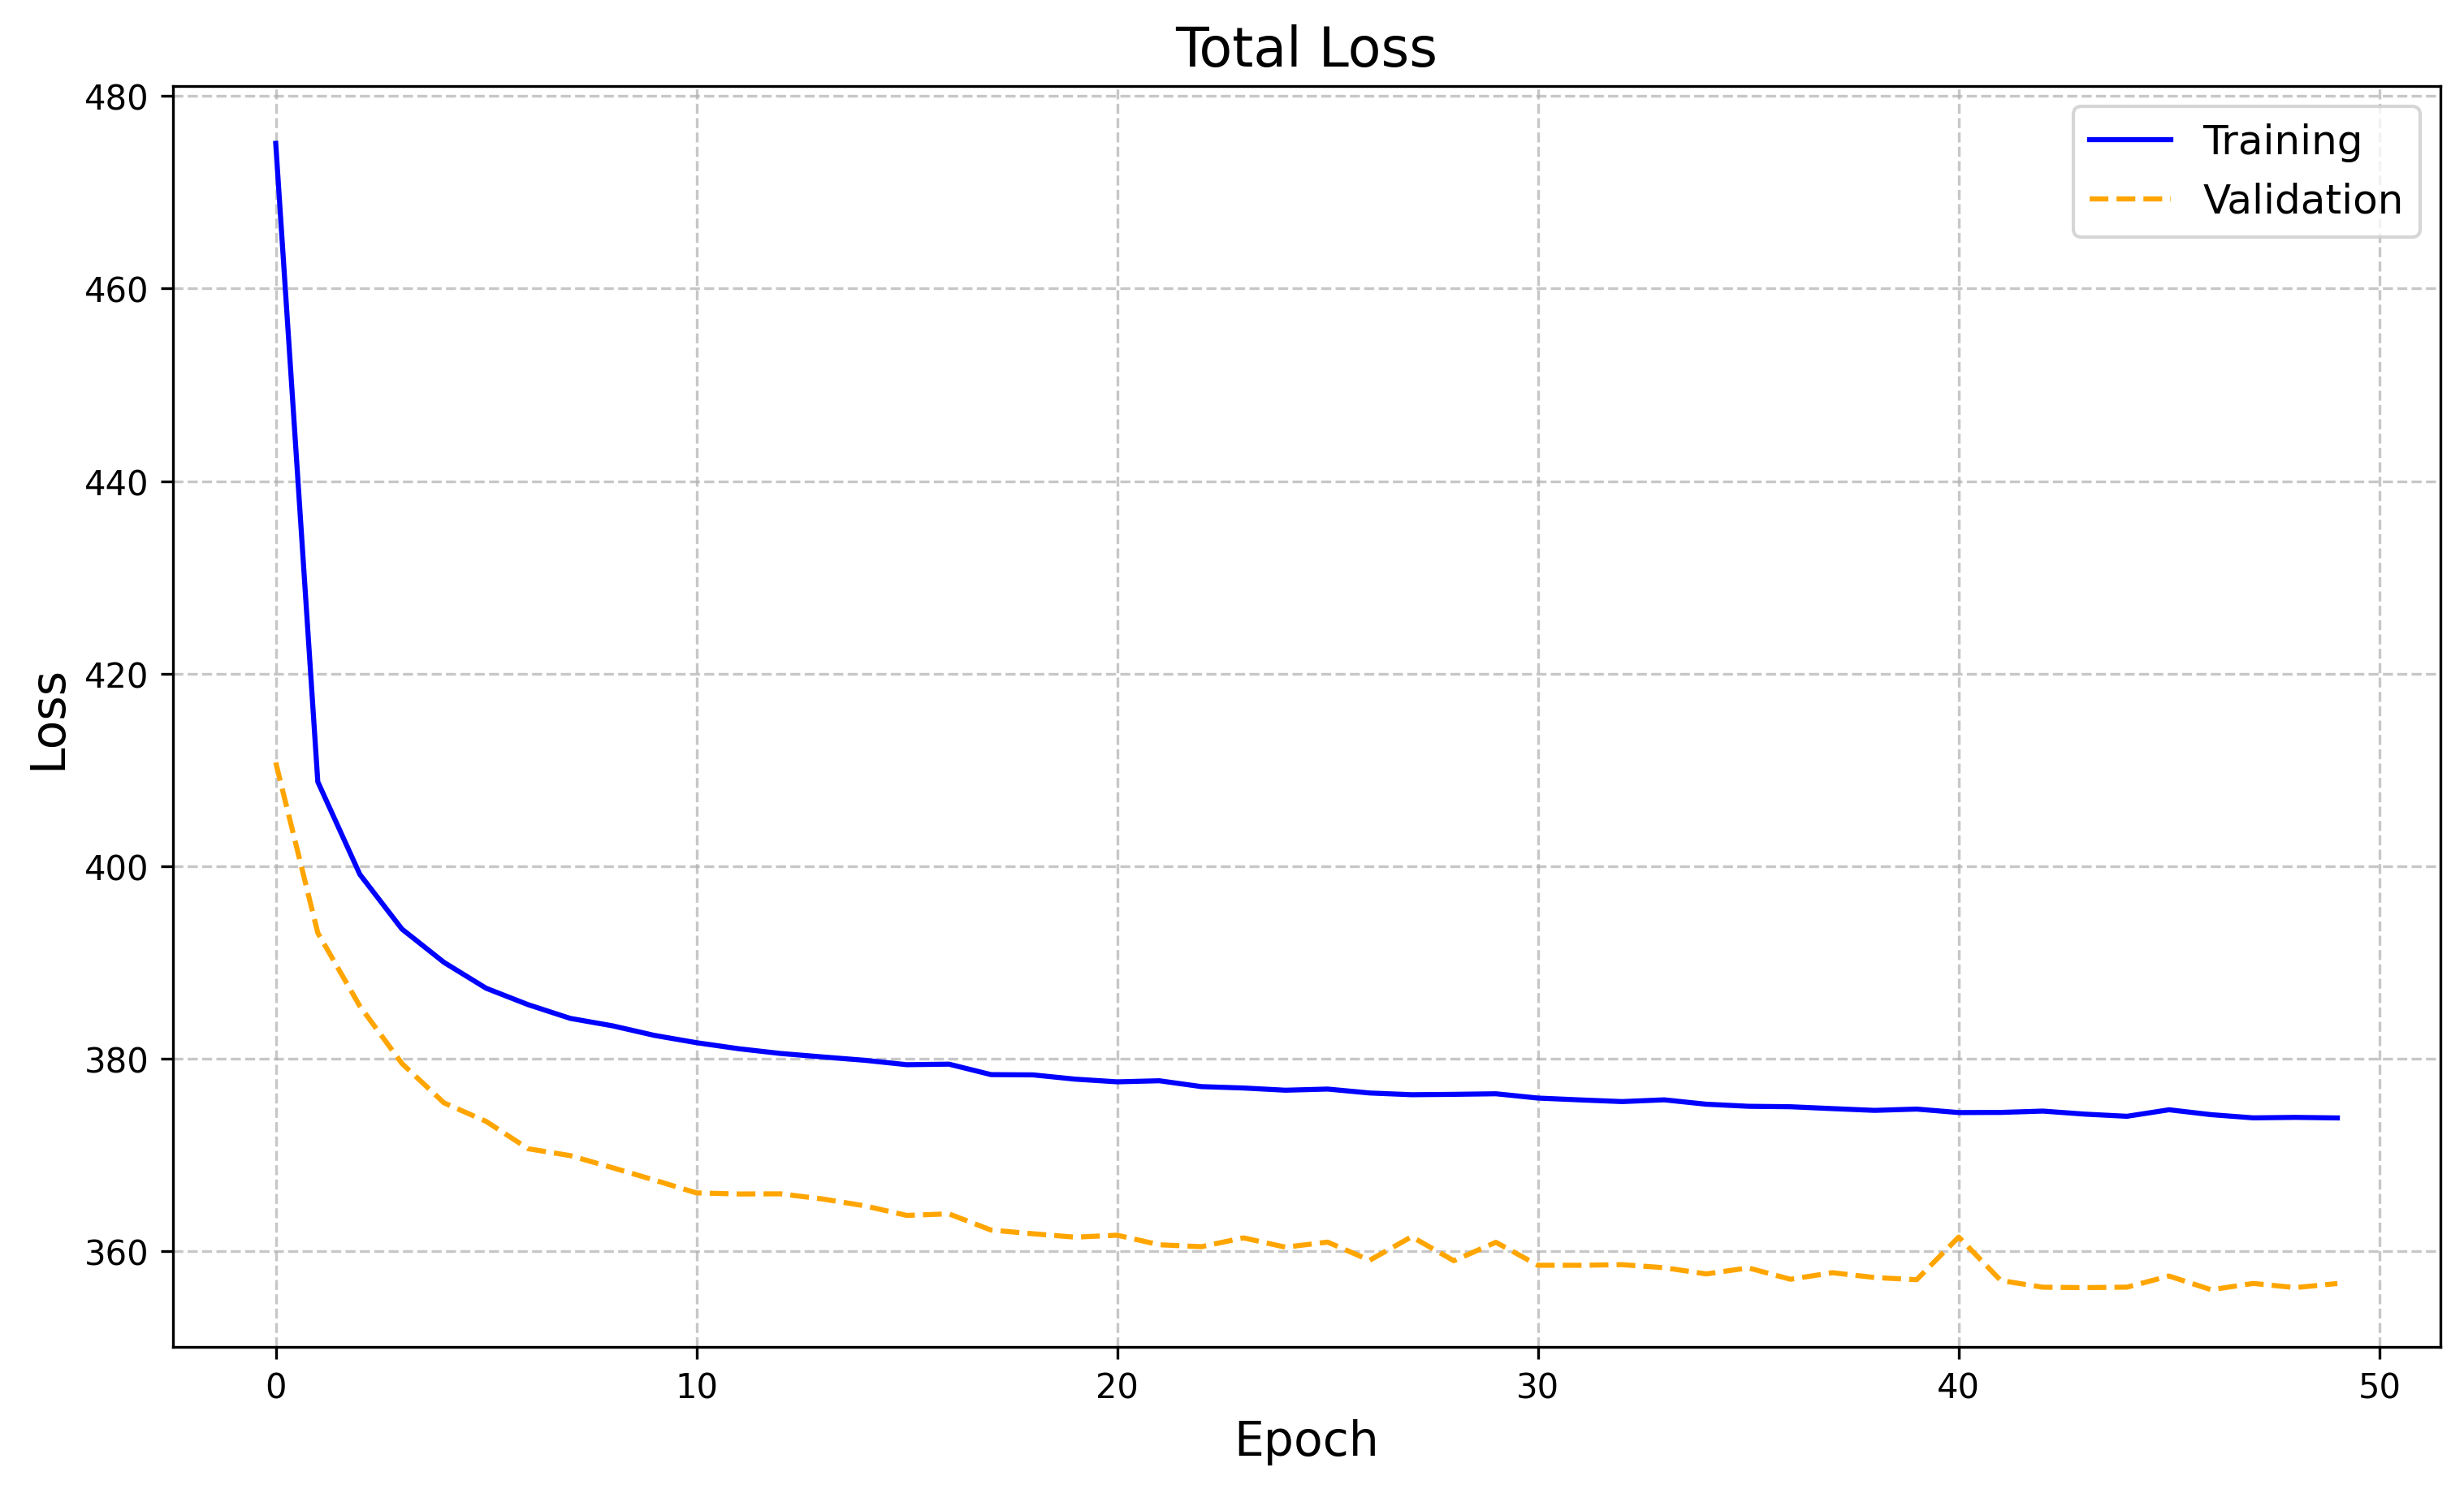
\includegraphics[width=0.8\textwidth]{total_loss.png}
\end{figure}

\begin{figure}[H]
    \centering
    \begin{subfigure}[b]{0.48\textwidth}
        \centering
        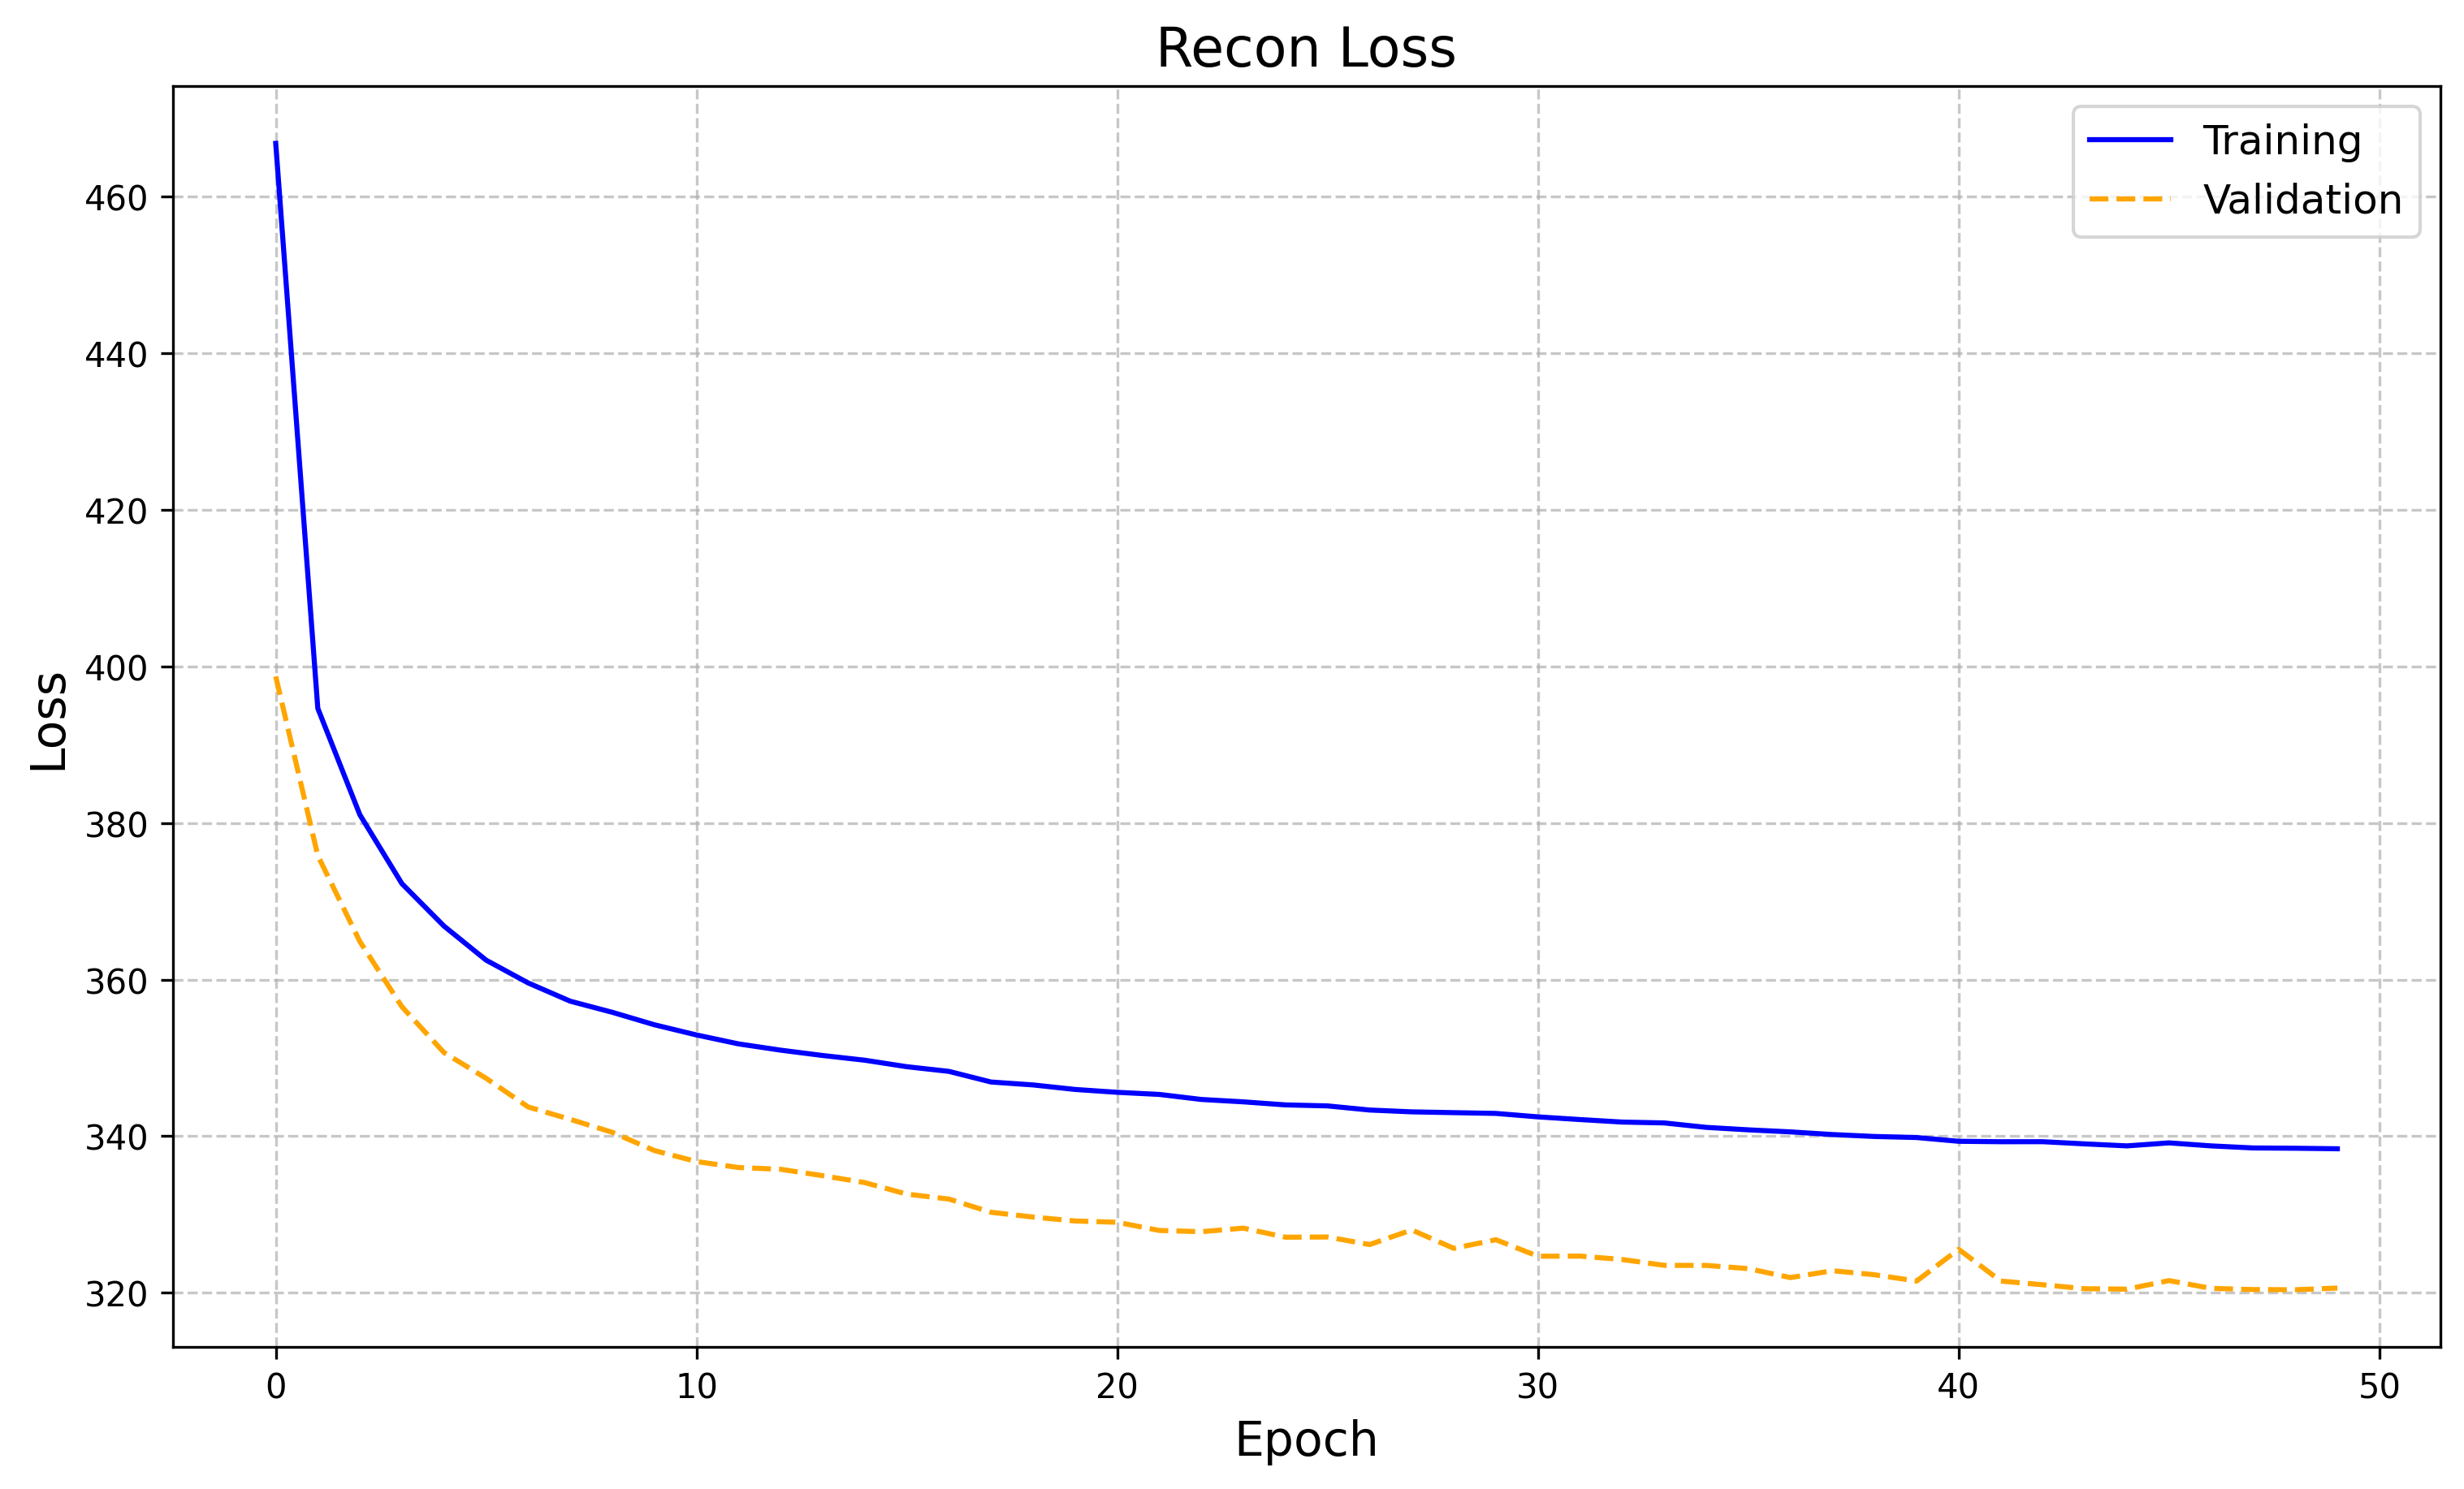
\includegraphics[width=\textwidth]{recon_loss.png}
    \end{subfigure}
    \hfill
    \begin{subfigure}[b]{0.48\textwidth}
        \centering
        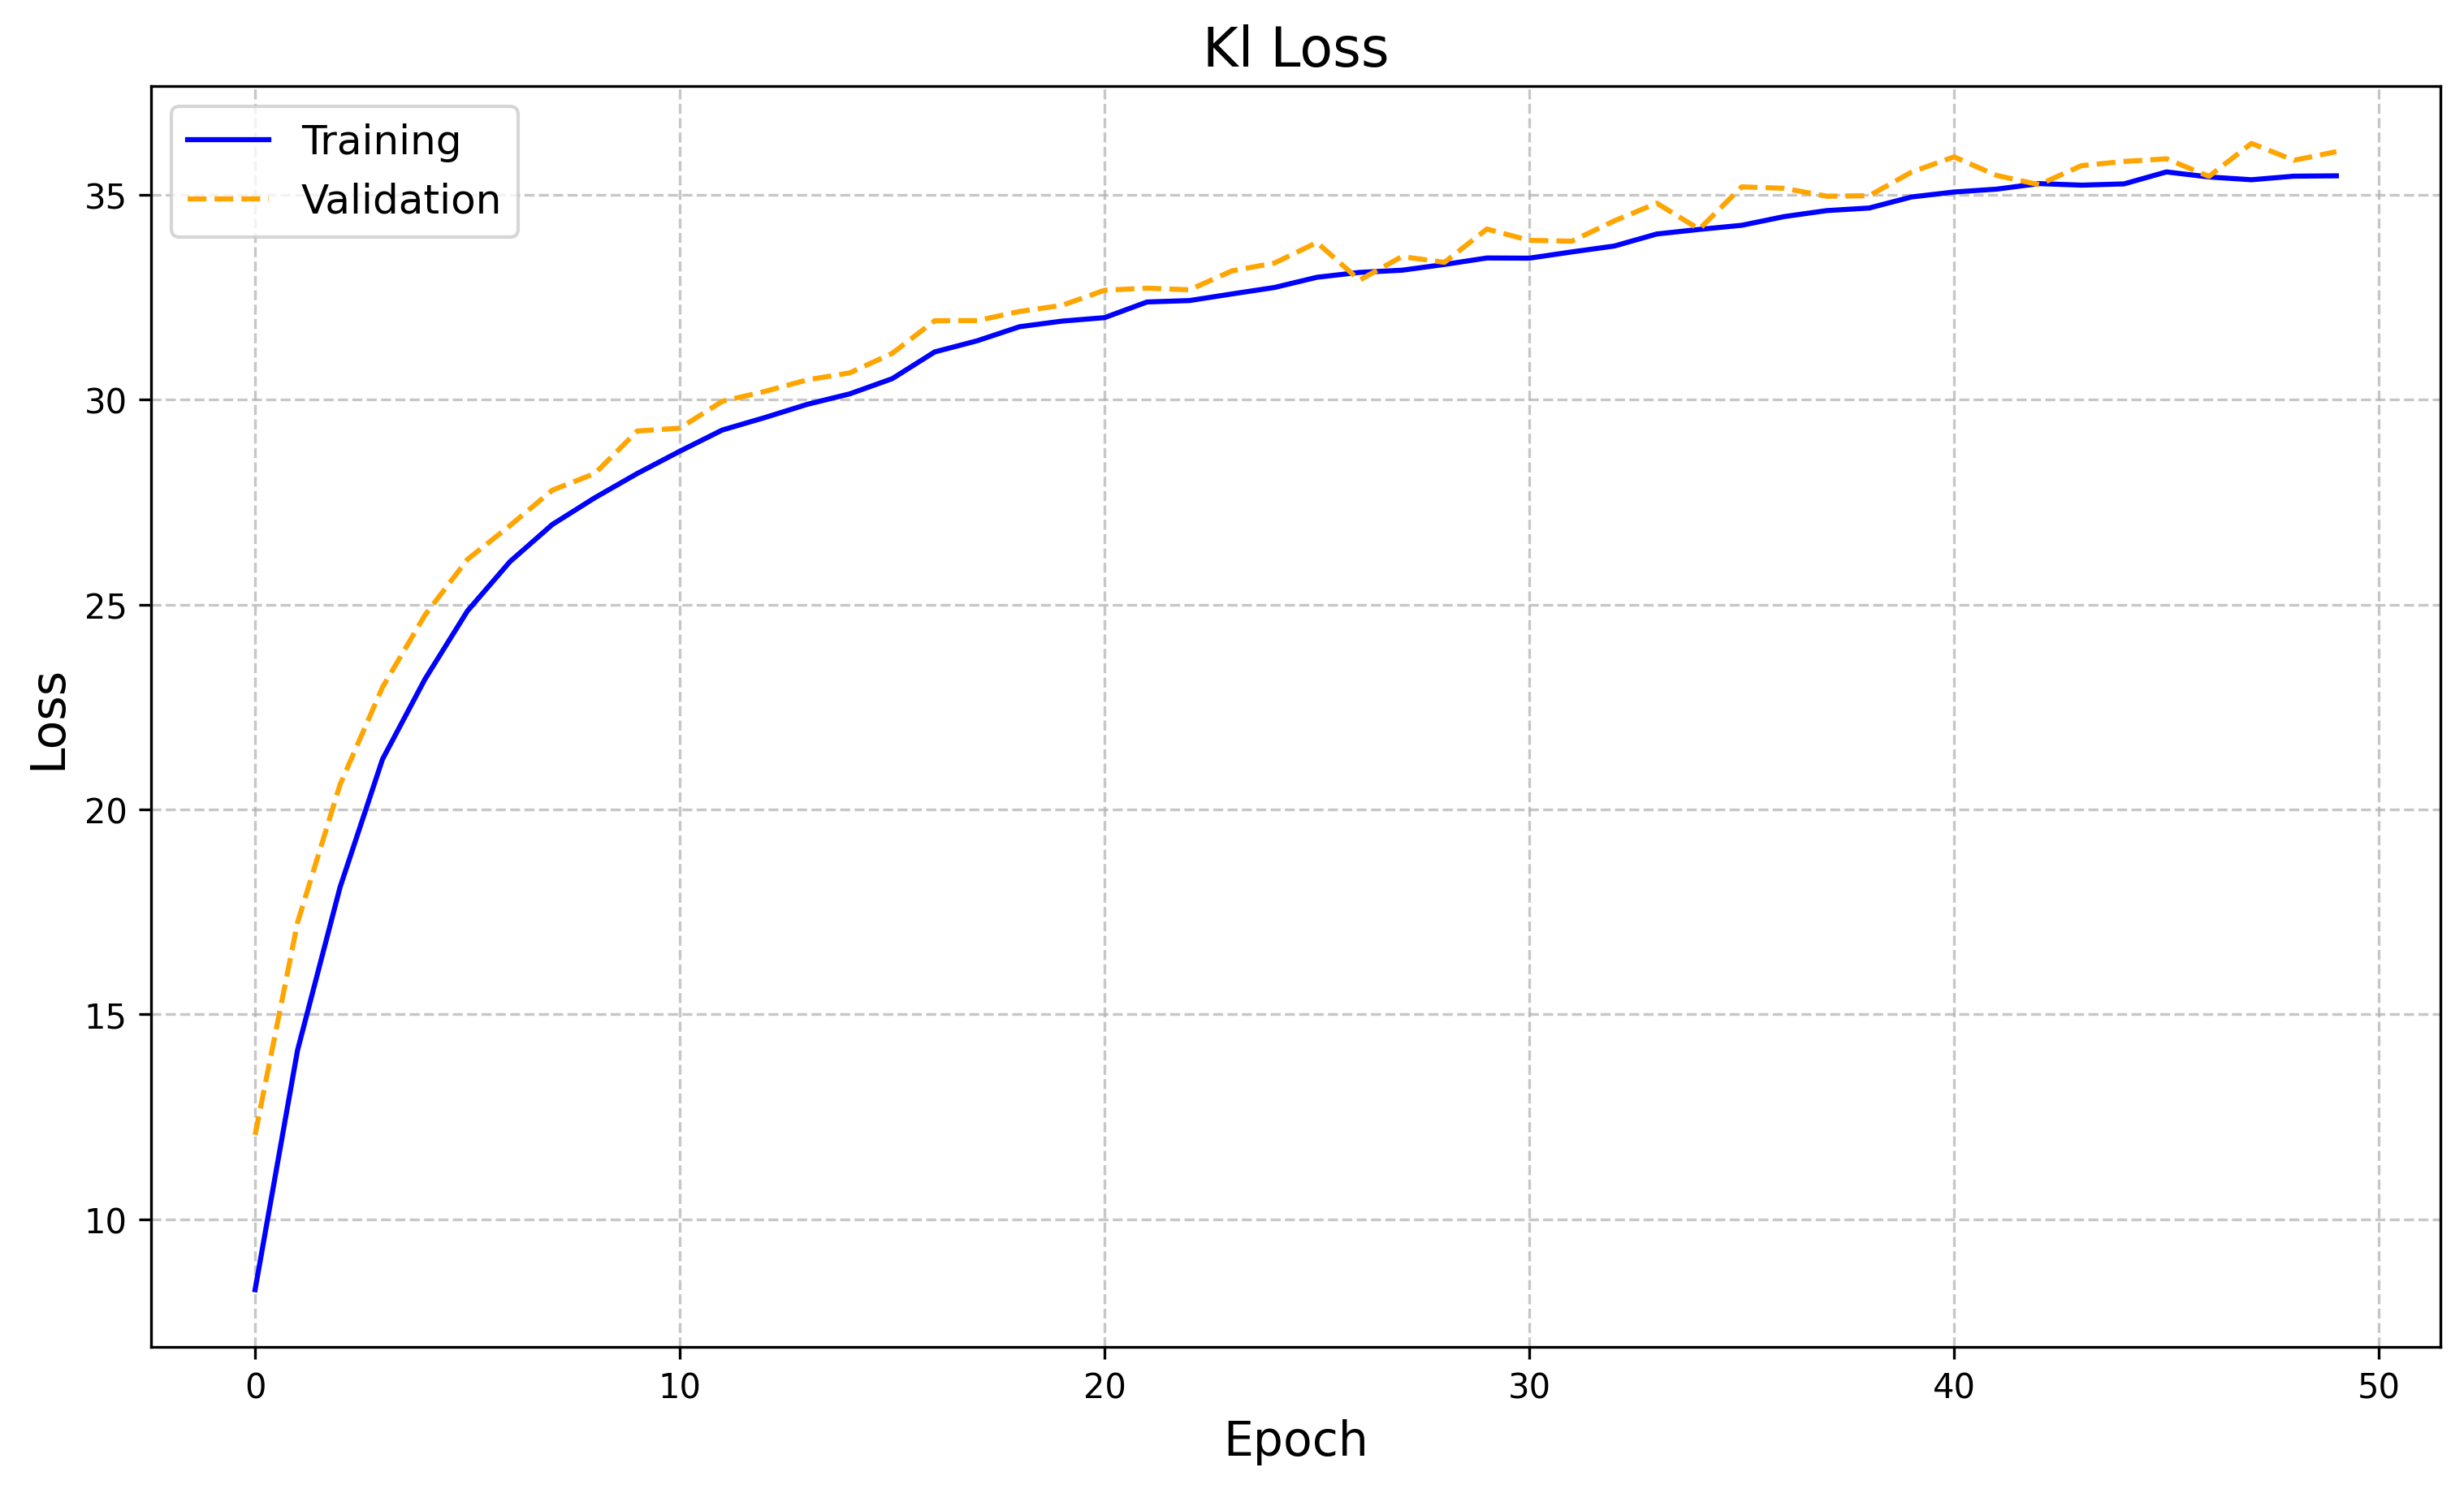
\includegraphics[width=\textwidth]{kl_loss.png}
    \end{subfigure}
\end{figure}

\subsection{Observables}
\begin{figure}[H]
    \centering
    \begin{subfigure}[b]{0.48\textwidth}
        \centering
        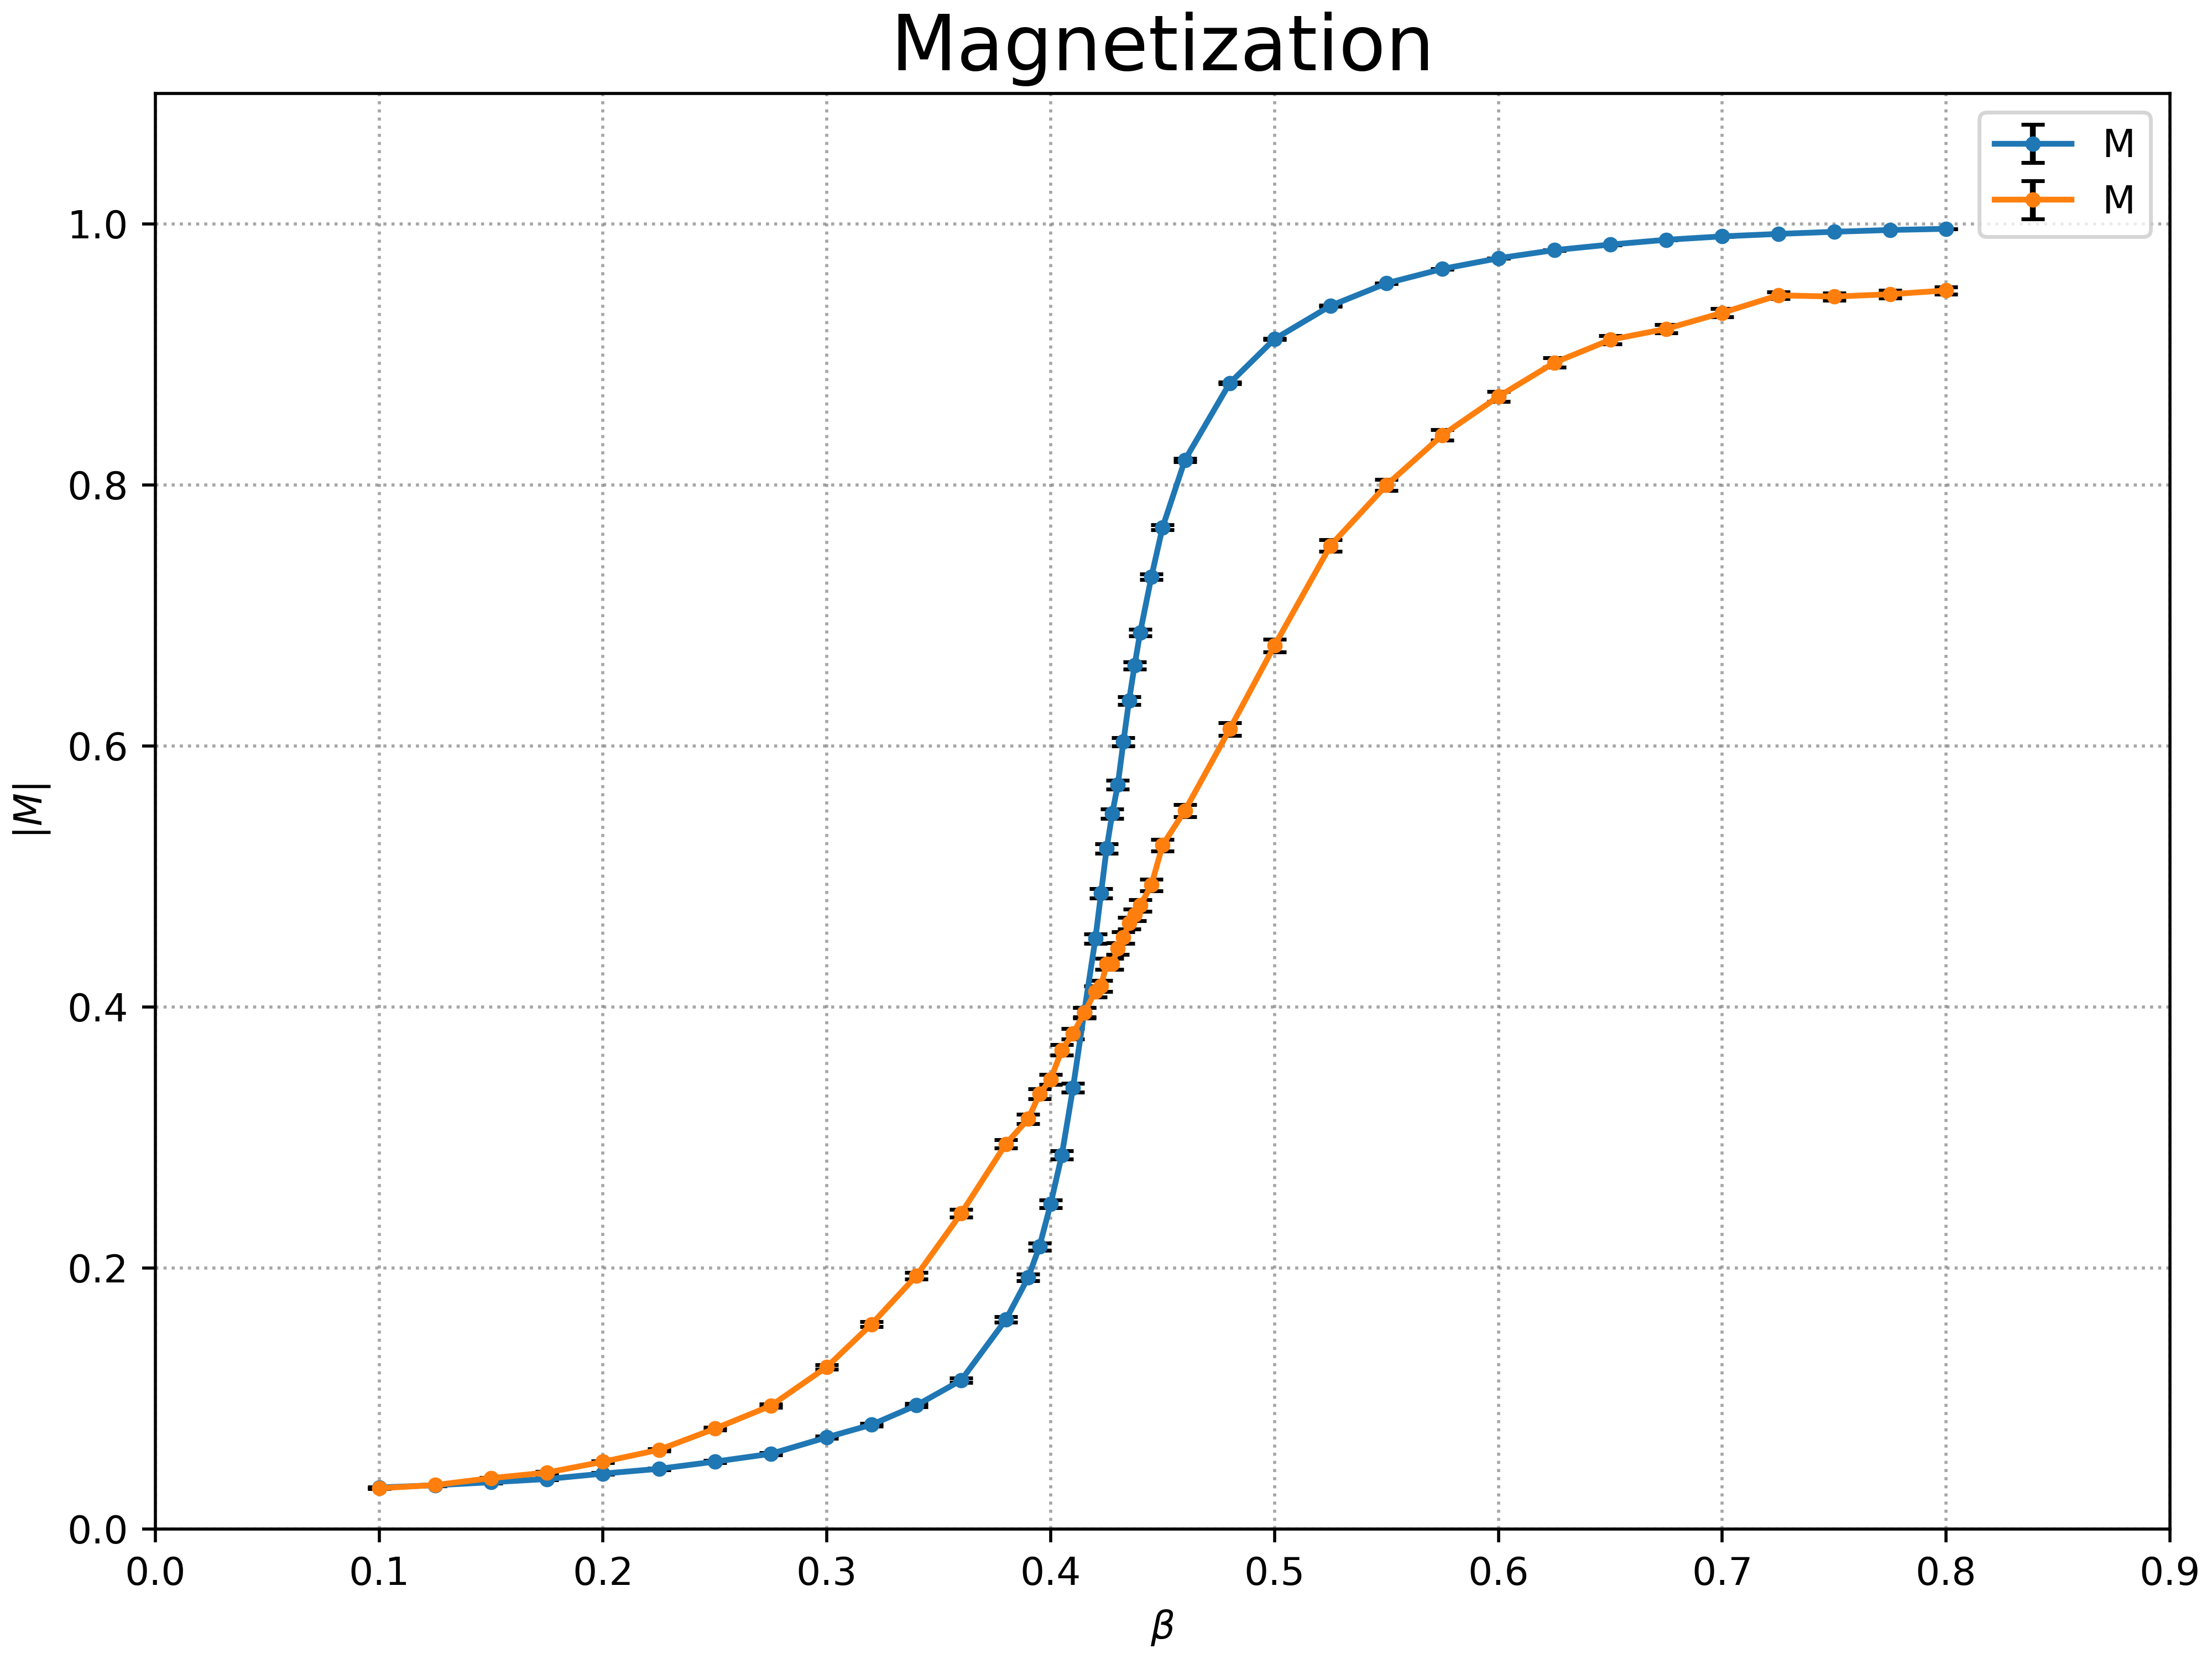
\includegraphics[width=\textwidth]{Magnetization.png}
        \caption{Mean Magnetization $\langle |M| \rangle$ vs $\beta$}
    \end{subfigure}
    \hfill
    \begin{subfigure}[b]{0.48\textwidth}
        \centering
        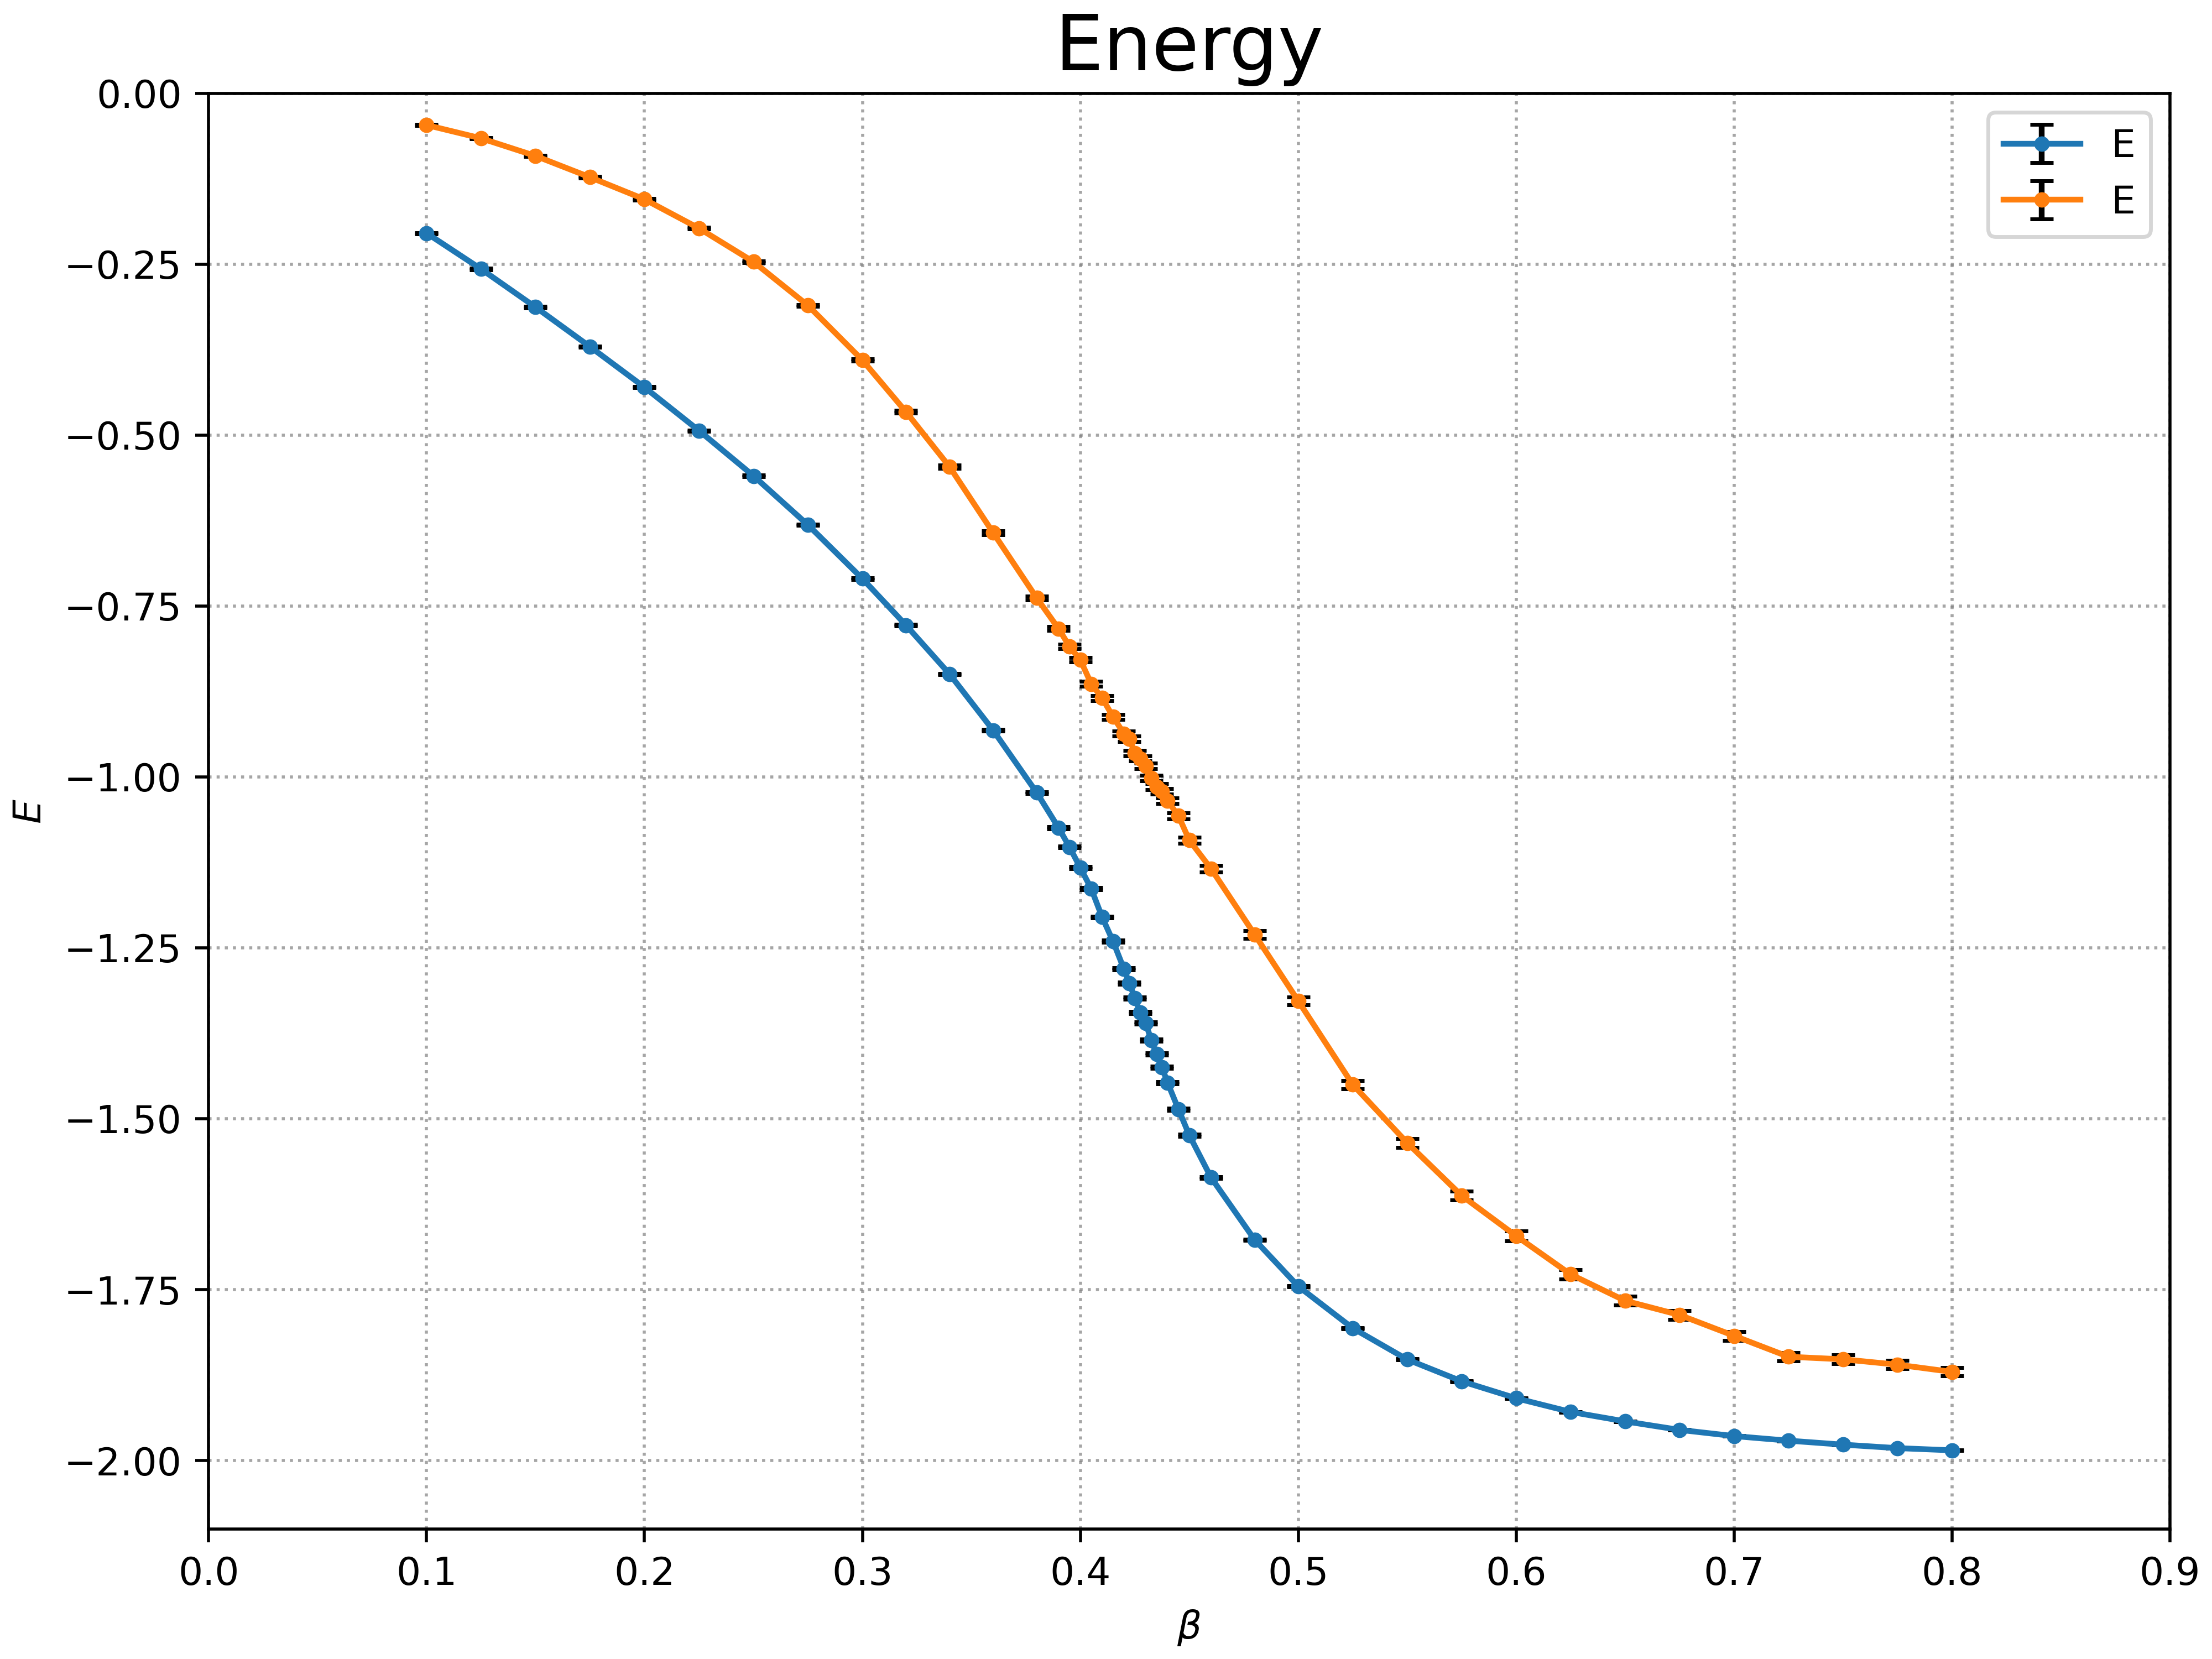
\includegraphics[width=\textwidth]{Energy.png}
        \caption{Mean Energy $\langle E \rangle$ vs $\beta$}
    \end{subfigure}
    \caption{Comparison of CVAE and Ising observables}
\end{figure}

\begin{figure}[H]
    \centering
    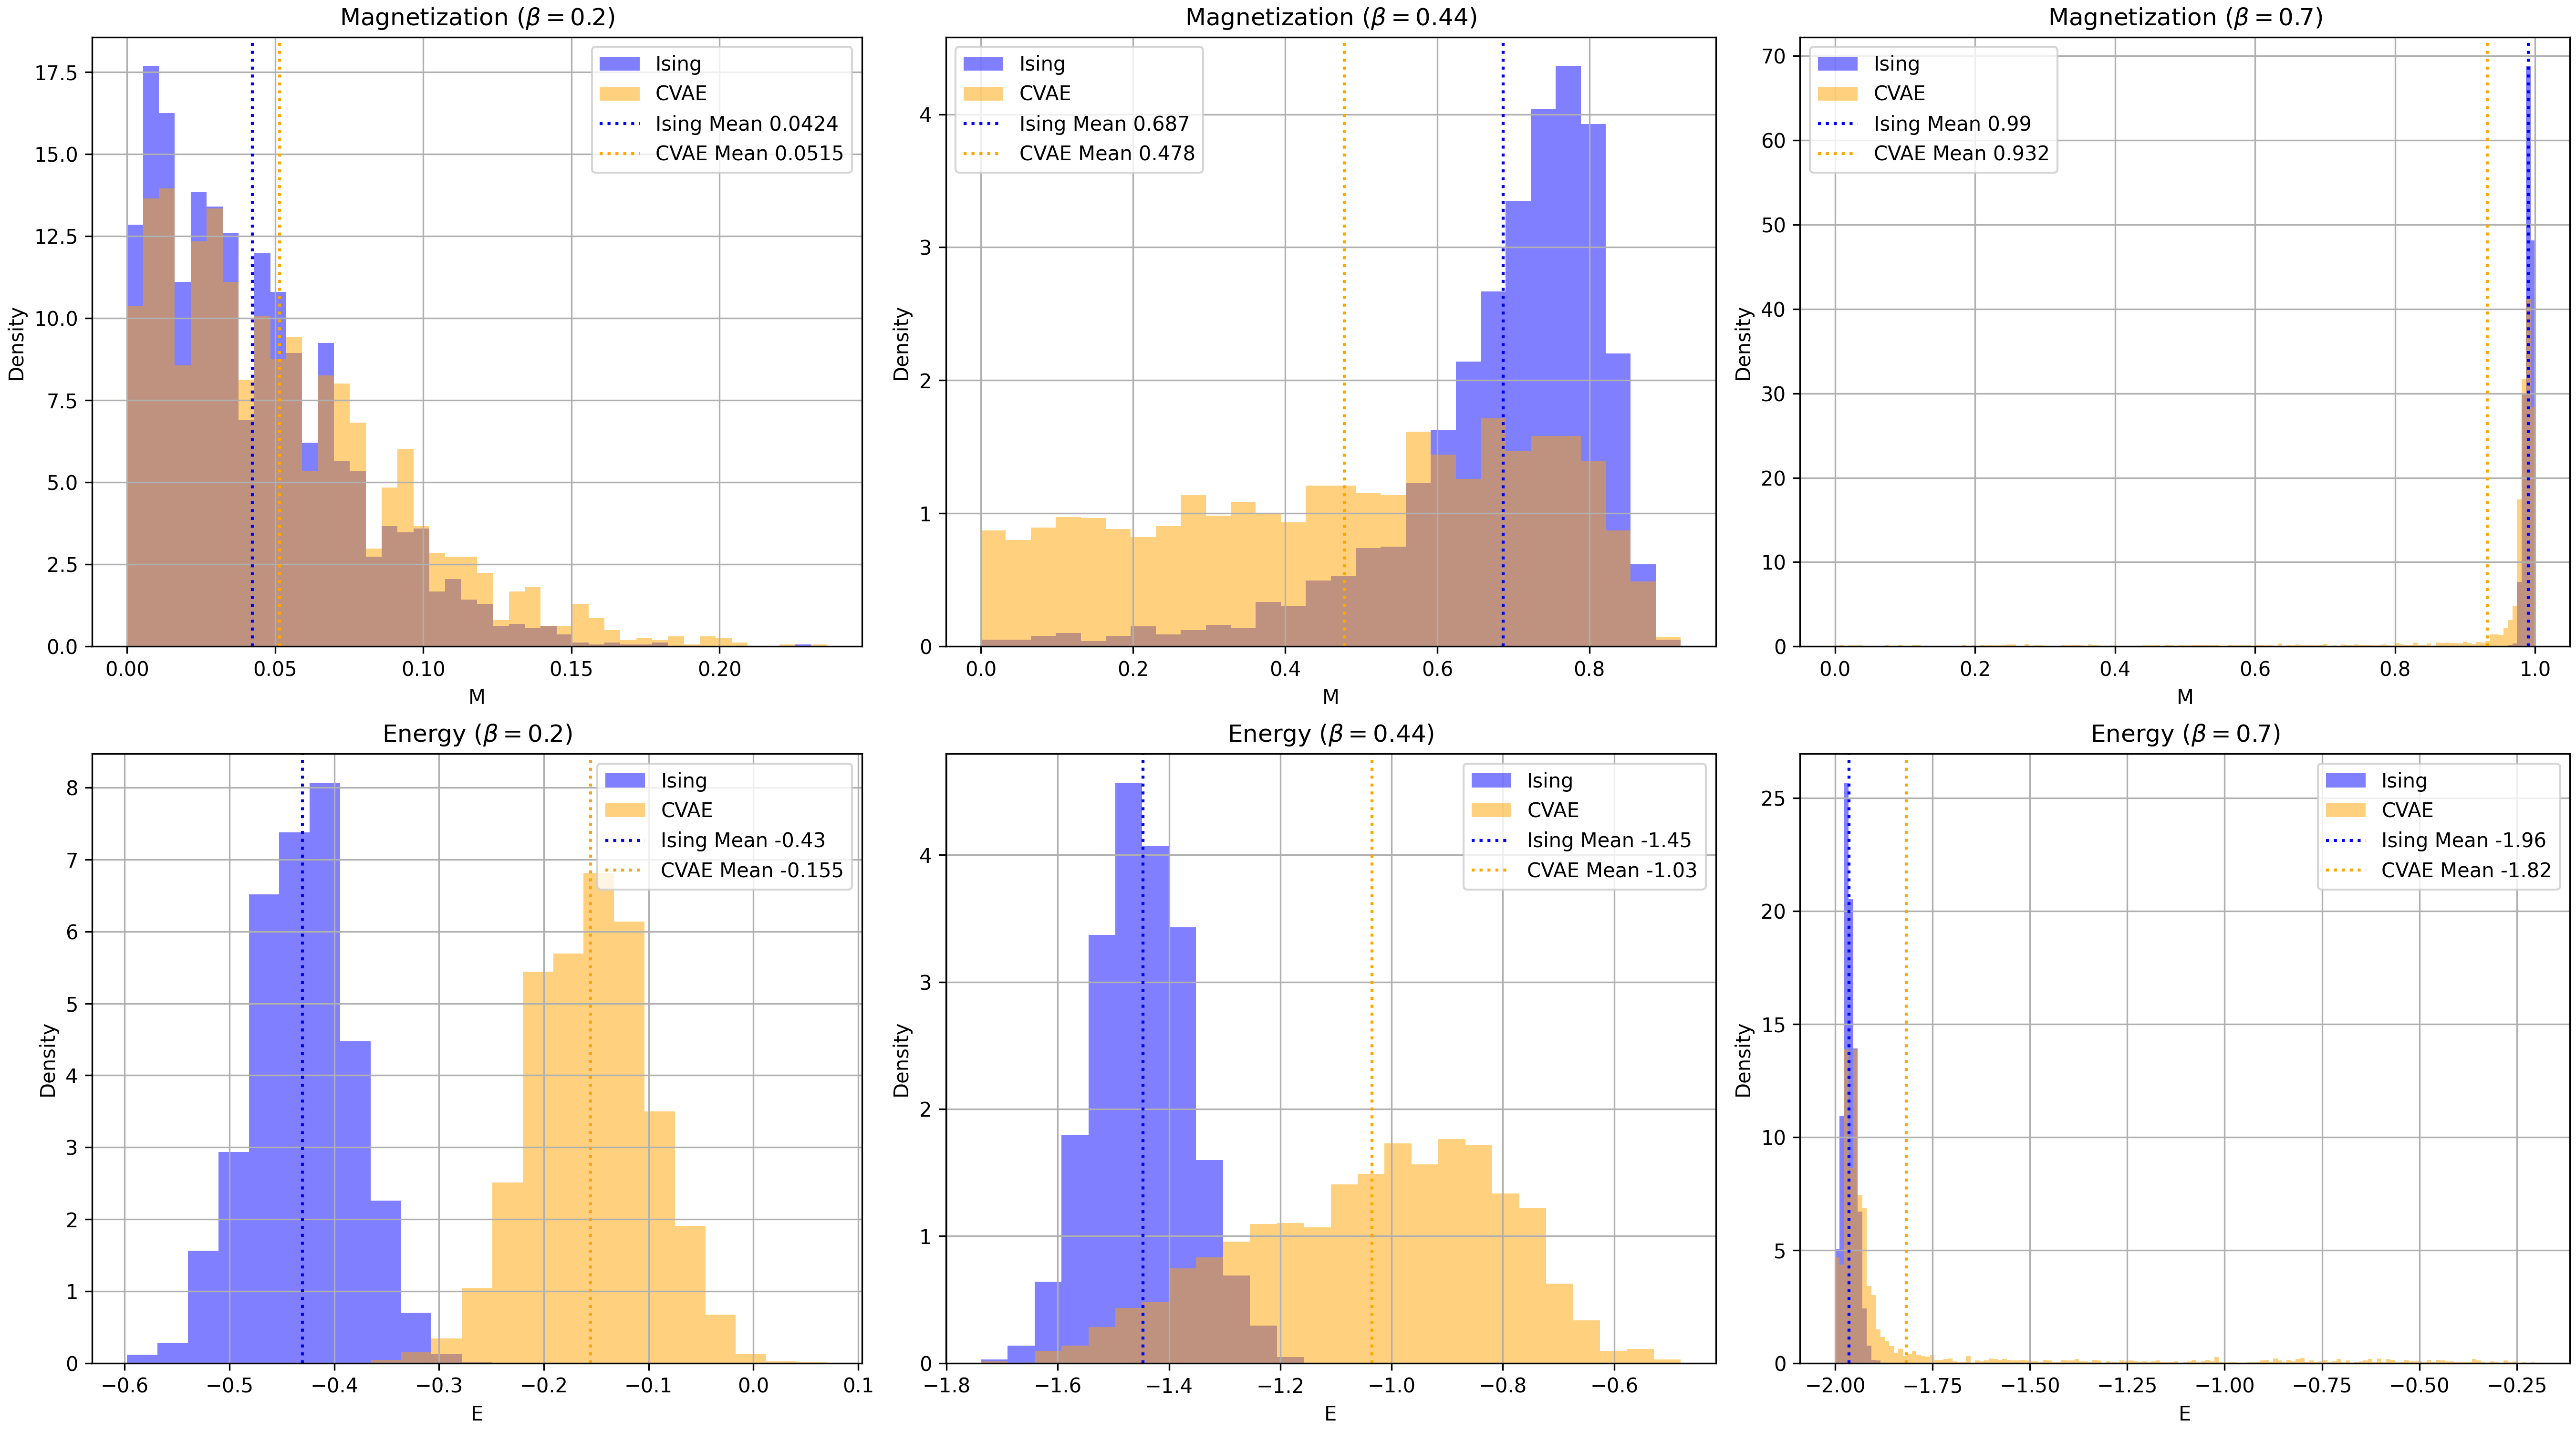
\includegraphics[width=0.8\textwidth]{histograms.png}
    \caption{Energy (Top) and Magnetization (Bottom) histograms for selected temperatures: 
             Disordered ($\beta=0.2$), Critical ($\beta=0.43$), and Ordered ($\beta=0.8$). The CVAE struggles 
             to capture the magnetization and energy distributions at low temperatures in a similar way,
             showing long tails that correspons to unphysical lattice configurations. At higher temperatures
             the energy is offet positivelty, showing the models inability to sharpley cature local correlations.}
\end{figure}

\section{Reconstructions}
\begin{figure}[H]
    \centering
    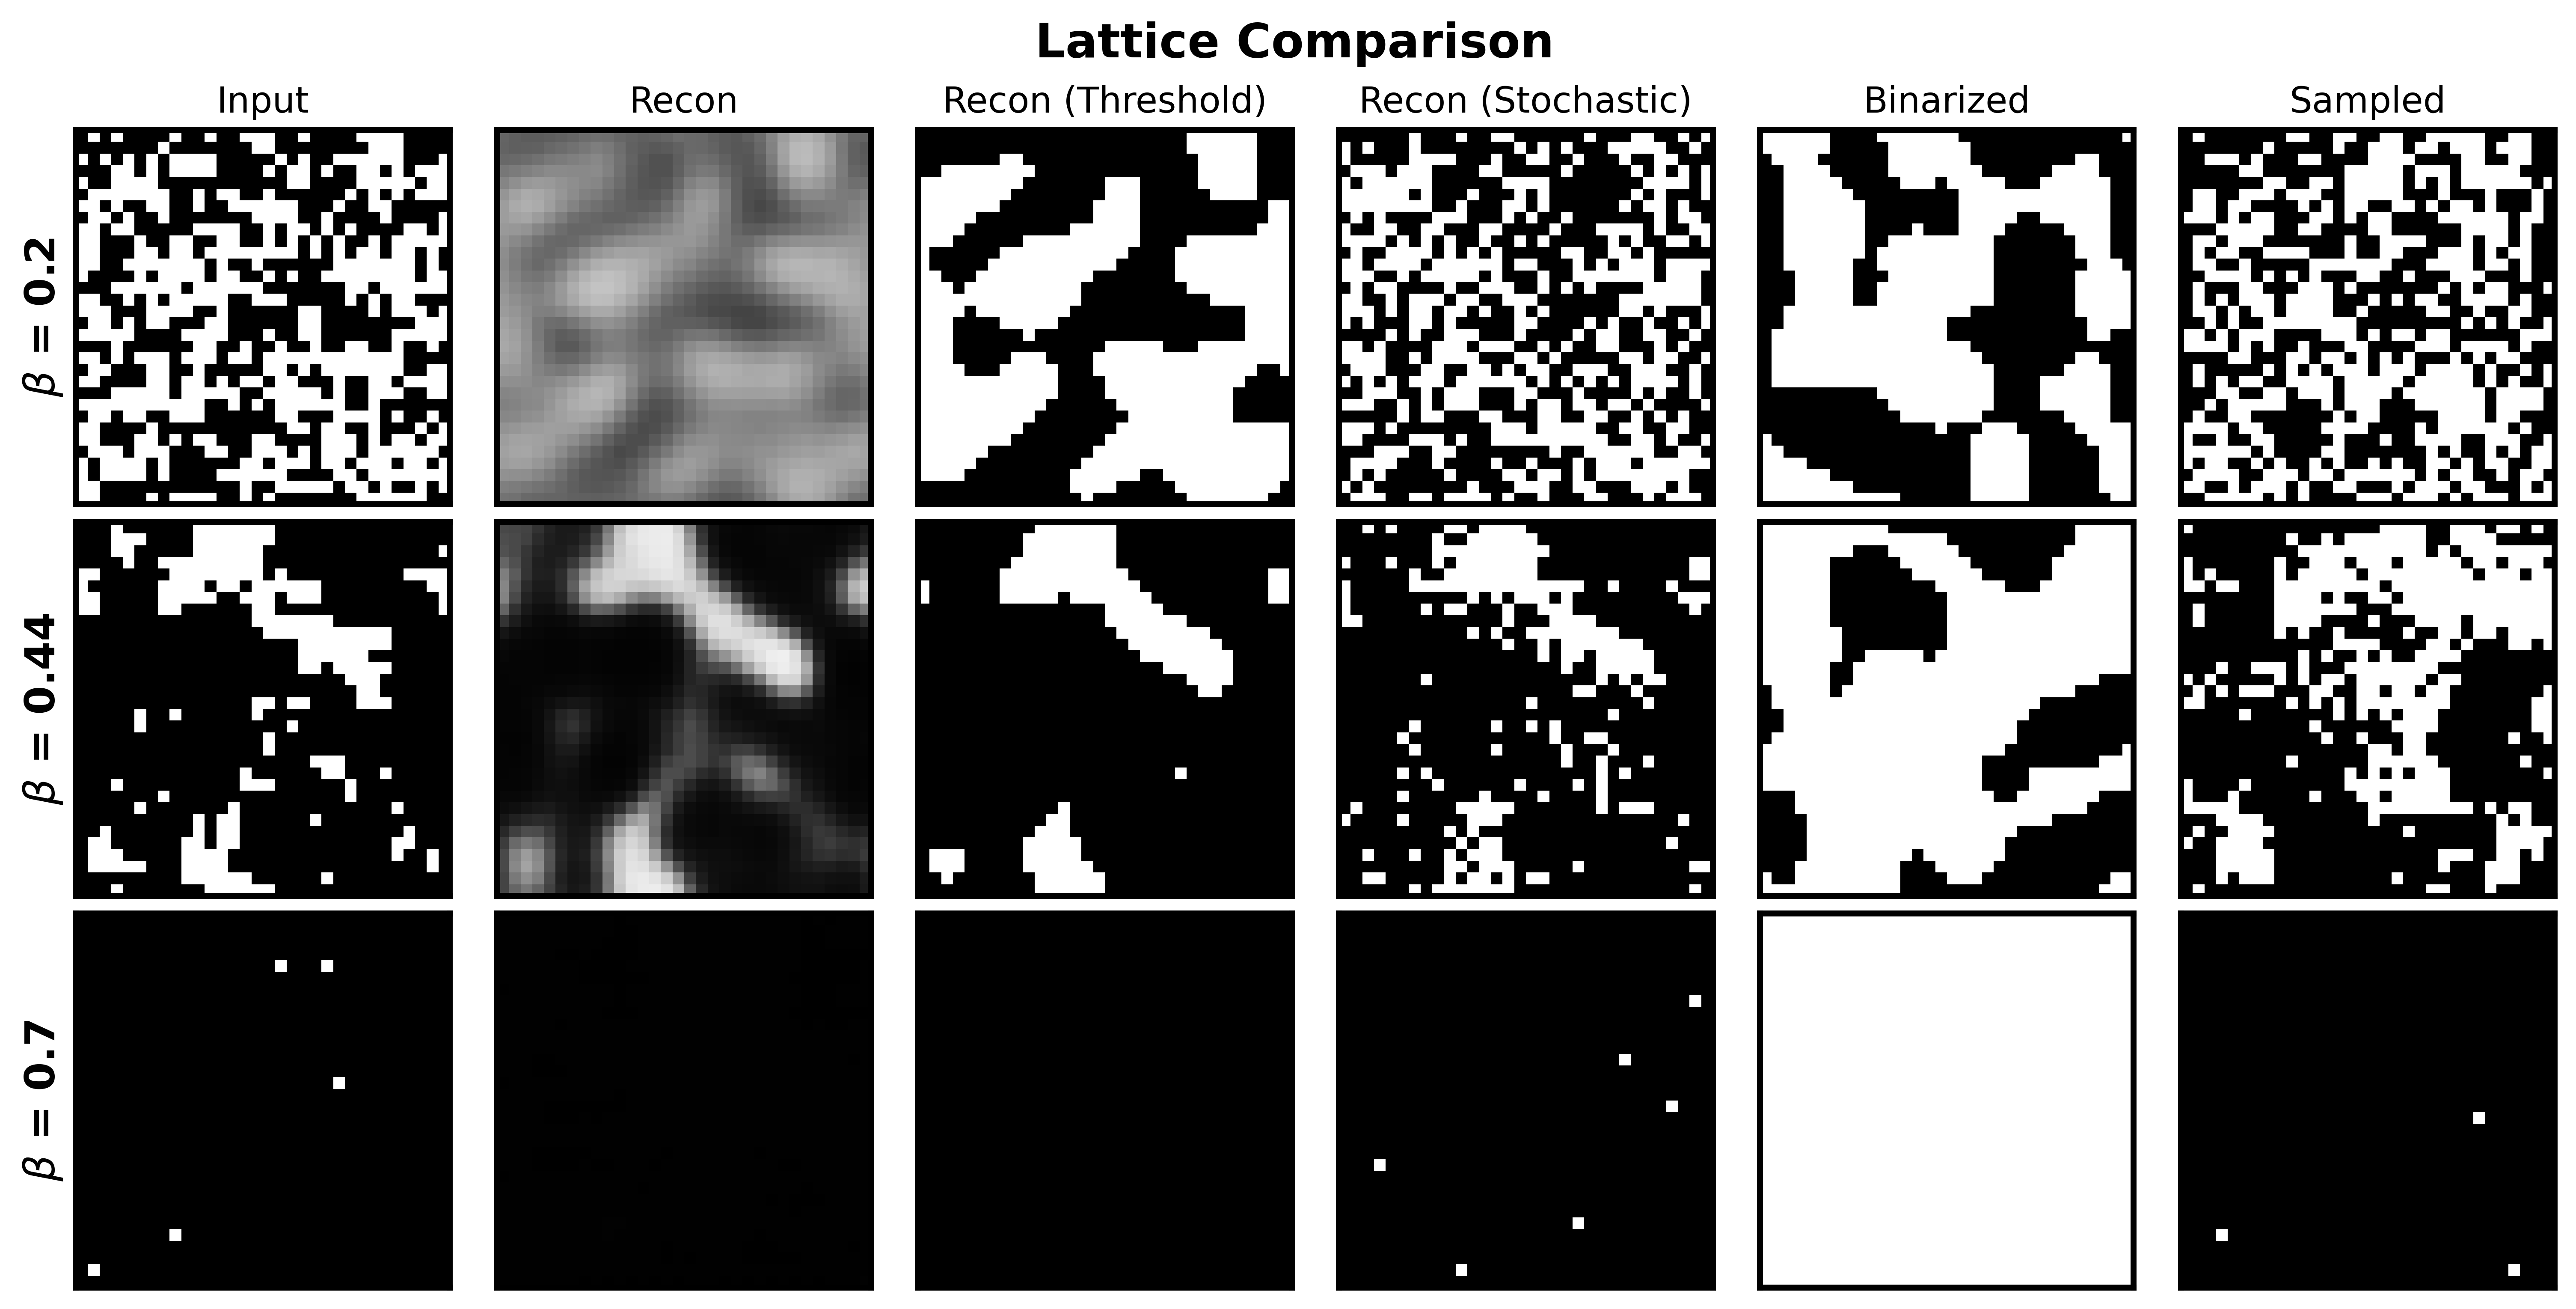
\includegraphics[width=0.9\textwidth]{reconstructions_combined.png}
    \caption{Input vs. Reconstructions for different phases: Disordered ($\beta=0.2$), Critical ($\beta=0.43$), and 
             Ordered ($\beta=0.8$). The reconstructions are for the float CVAE output, binarized ouput, stochastically 
             sampled binary outpt, and the CVAE generated binarized and stochastic outputs.}
\end{figure}

\begin{figure}[H]
    \centering
    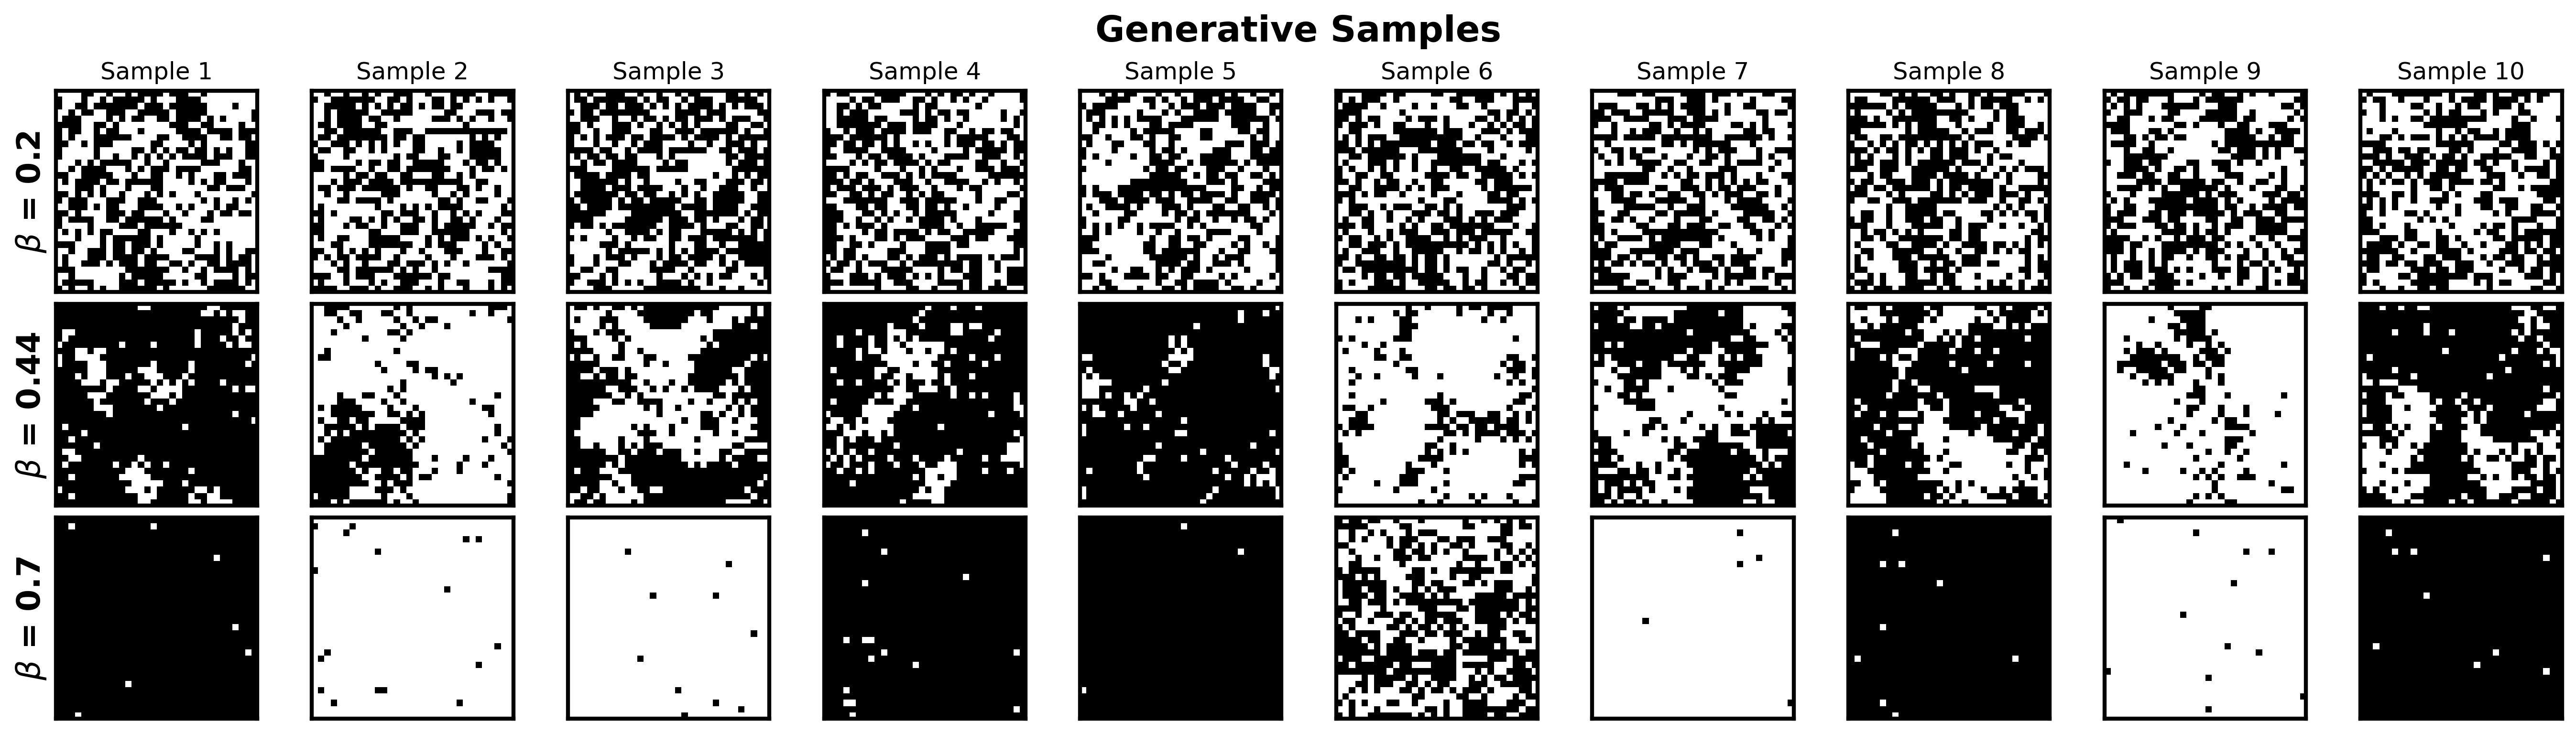
\includegraphics[width=0.9\textwidth]{recon_samples.png}
\end{figure}




\end{document}
